% Taxonomy of compression techniques drawn in TikZ.
% 4 columns on top row, 3 columns on bottom row.
\definecolor{famBlue}{RGB}{31,119,180}
\definecolor{famGreen}{RGB}{44,160,44}
\definecolor{famRed}{RGB}{214,39,40}
\definecolor{famPurple}{RGB}{148,103,189}
\definecolor{famOrange}{RGB}{255,127,14}
\definecolor{famBrown}{RGB}{140,86,75}
\definecolor{famTeal}{RGB}{23,190,207}

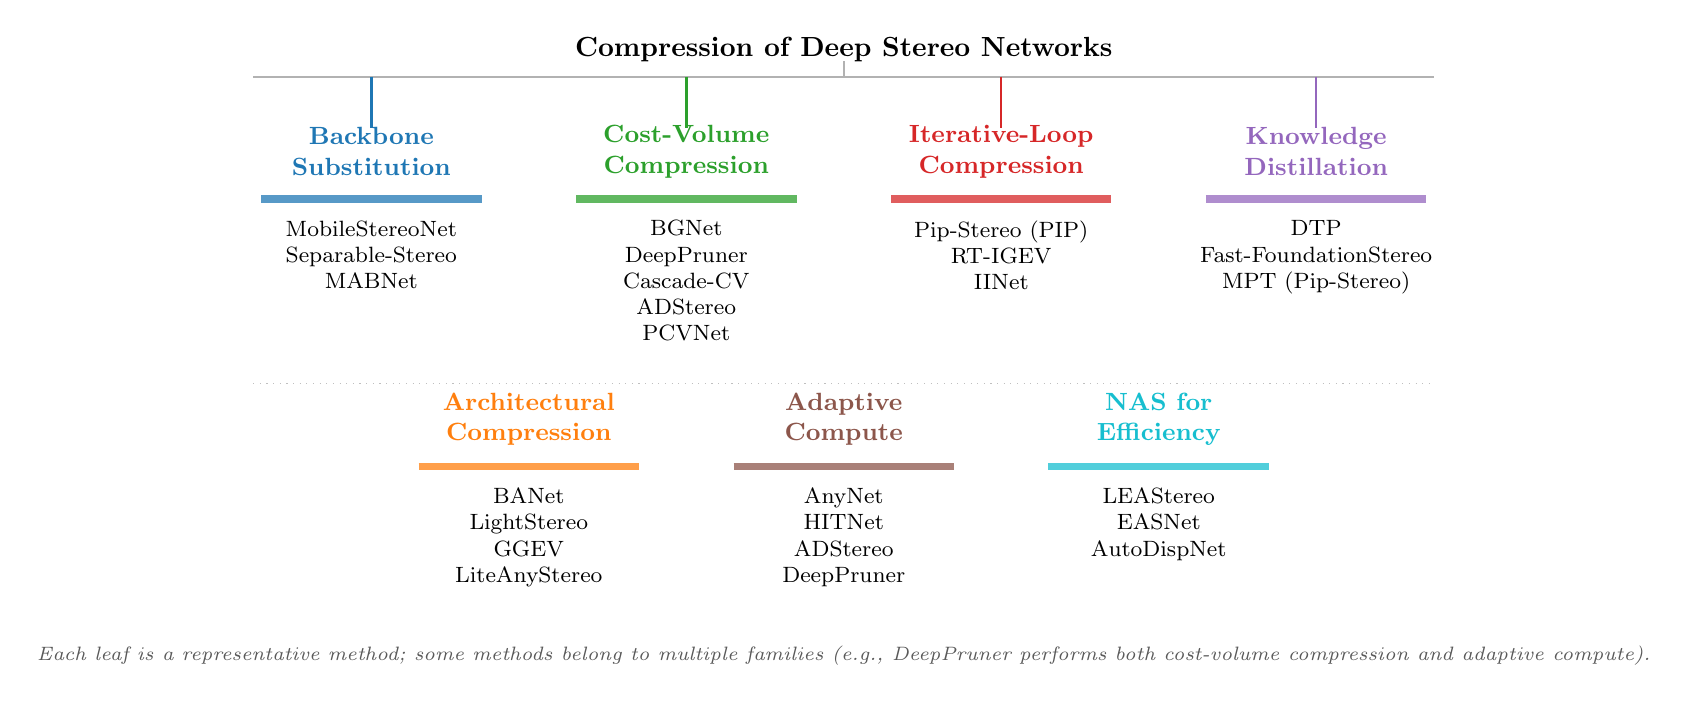
\begin{tikzpicture}[
  every node/.style = {font=\small},
  root/.style = {font=\bfseries},
  branch/.style = {line width=0.9pt, draw=gray!60},
  famheader/.style = {font=\bfseries\small, align=center,
                      text width=3.4cm, inner sep=2pt},
  rail/.style = {line width=2.8pt, draw opacity=0.75},
  methodlist/.style = {font=\footnotesize, align=center,
                       text width=3.2cm, inner sep=2pt}
]

% --- Root and trunk ---
\node[root] (root) at (0, 6.2) {Compression of Deep Stereo Networks};
\draw[branch] (-7.5, 5.85) -- (7.5, 5.85);
\draw[branch] (0, 6.05) -- (0, 5.85);

% ================= TOP ROW =================
% Backbone Substitution
\draw[branch, draw=famBlue] (-6.0, 5.85) -- (-6.0, 5.2);
\node[famheader, text=famBlue] at (-6.0, 4.9) {Backbone\\Substitution};
\draw[rail, draw=famBlue] (-7.4, 4.3) -- (-4.6, 4.3);
\node[methodlist, anchor=north] at (-6.0, 4.1)
  {MobileStereoNet \\ Separable-Stereo \\ MABNet};

% Cost-Volume Compression
\draw[branch, draw=famGreen] (-2.0, 5.85) -- (-2.0, 5.2);
\node[famheader, text=famGreen] at (-2.0, 4.9) {Cost-Volume\\Compression};
\draw[rail, draw=famGreen] (-3.4, 4.3) -- (-0.6, 4.3);
\node[methodlist, anchor=north] at (-2.0, 4.1)
  {BGNet \\ DeepPruner \\ Cascade-CV \\ ADStereo \\ PCVNet};

% Iterative-Loop Compression
\draw[branch, draw=famRed] (2.0, 5.85) -- (2.0, 5.2);
\node[famheader, text=famRed] at (2.0, 4.9) {Iterative-Loop\\Compression};
\draw[rail, draw=famRed] (0.6, 4.3) -- (3.4, 4.3);
\node[methodlist, anchor=north] at (2.0, 4.1)
  {Pip-Stereo (PIP) \\ RT-IGEV \\ IINet};

% Knowledge Distillation
\draw[branch, draw=famPurple] (6.0, 5.85) -- (6.0, 5.2);
\node[famheader, text=famPurple] at (6.0, 4.9) {Knowledge\\Distillation};
\draw[rail, draw=famPurple] (4.6, 4.3) -- (7.4, 4.3);
\node[methodlist, anchor=north] at (6.0, 4.1)
  {DTP \\ Fast-FoundationStereo \\ MPT (Pip-Stereo)};

% --- Divider between rows ---
\draw[dotted, gray!50] (-7.5, 1.95) -- (7.5, 1.95);

% ================= BOTTOM ROW =================
% Architectural Compression
\node[famheader, text=famOrange] at (-4.0, 1.5) {Architectural\\Compression};
\draw[rail, draw=famOrange] (-5.4, 0.9) -- (-2.6, 0.9);
\node[methodlist, anchor=north] at (-4.0, 0.7)
  {BANet \\ LightStereo \\ GGEV \\ LiteAnyStereo};

% Adaptive Compute
\node[famheader, text=famBrown] at (0, 1.5) {Adaptive\\Compute};
\draw[rail, draw=famBrown] (-1.4, 0.9) -- (1.4, 0.9);
\node[methodlist, anchor=north] at (0, 0.7)
  {AnyNet \\ HITNet \\ ADStereo \\ DeepPruner};

% NAS for Efficiency
\node[famheader, text=famTeal] at (4.0, 1.5) {NAS for\\Efficiency};
\draw[rail, draw=famTeal] (2.6, 0.9) -- (5.4, 0.9);
\node[methodlist, anchor=north] at (4.0, 0.7)
  {LEAStereo \\ EASNet \\ AutoDispNet};

% Footer
\node[align=center, font=\scriptsize\itshape, text=gray!70!black]
  at (0, -1.5) {Each leaf is a representative method; some methods belong to multiple families (e.g., DeepPruner performs both cost-volume compression and adaptive compute).};

\end{tikzpicture}
